% Author Vahid Partovi Nia
% Copyright Huawei Technologies
% Network Mind Team



\documentclass[12pt]{beamer}

\usetheme{Hannover}
\setbeamercolor{section in sidebar shaded}{fg=black}

\usecolortheme{beaver}
\beamertemplatenavigationsymbolsempty

%  \usebeamertemplate{navigation symbols}\hfill
%  \insertframenumber{}/\inserttotalframenumber}
  

\useoutertheme{sidebar}
\pgfdeclareimage[width=2.5\baselineskip]{institut-logo}{fig/mcgill_logo}
\setbeamertemplate{footline}
{\raisebox{-2ex}{\pgfuseimage{institut-logo}}
%  \hfill
\hspace{5cm}
  \usebeamertemplate{navigation symbols}
  \insertframenumber{}/\inserttotalframenumber
  \hspace{3.8cm}
YCBS255
}
%\setbeamertemplate{sidebar right}{}
  
\setbeamercolor{block title}{fg=darkred}
\setbeamercolor{local structure}{fg=darkred}

\setbeamercolor{palette sidebar secondary}{fg=darkgray, bg=white}



\usefonttheme{professionalfonts} % using non standard fonts for beamer


\makeatletter
\beamer@nav@subsectionstyle{hide/hide/hide}
\makeatother

\titlegraphic{
\includegraphics[width=2cm]{fig/mcgill_logo}}




\usepackage{listings}
\usepackage{xcolor}
\def \y {\mathbf y}
\def \z {\mathbf z}
\def \Z {\mathbf Z}
\def \X {\mathbf X}
\def \A {\mathbf A}
\def \t {^\top}
\def \inv {^ {-1}}
\def \x {\mathbf x}
\def \bbeta {\boldsymbol \beta}
\def \eeps {\boldsymbol \varepsilon}
\def \TV {\mathrm{TV}}
\def \Radio {\mathrm{Radio}}
\def \Newspaper {\mathrm{Newspaper}}
\def \Sales {\mathrm{Sales}}
\def \Balance {\mathrm{Balance}}
\def \Default {\mathrm{Default}}
\def \M {\mathcal{M}}

\def \r {\mathbf{r}}
\def \e {\mathbf{e}}

\def \RSS {\mathrm{RSS}}

\def \E {\mathrm{E}}
\def \P {\mathbf{P}}

\def \V {\mathrm{V}}
\def \cor {\mathrm{cor}}

\def \SSigma {\boldsymbol{\Sigma}}
\def \LLambda {\boldsymbol{\Lambda}}
\def \pphi {\boldsymbol{\phi}}
\def \PPhi {\boldsymbol{\Phi}}
\def \mmu {\boldsymbol{\mu}}
\def \ttheta {\boldsymbol{\theta}}


\definecolor{capri}{rgb}{0.0, 0.75, 1.0}
\definecolor{darkcyan}{rgb}{0.0, 0.55, 0.55}
\definecolor{deepfuchsia}{rgb}{0.76, 0.33, 0.76}

\begin{document}
% no title and no author on sidebar
\title[]{Powerful Classifiers}   
\author[]{Vahid Partovi Nia} 
\institute{Lecture 09}
\date{}


\makeatletter
  \begin{frame}[plain]
    \hspace*{-\beamer@leftsidebar}%
    \advance\textwidth by \beamer@leftsidebar\relax
    \beamer@leftsidebar=\z@
    \begin{minipage}{\textwidth}\par%
      \maketitle
    \end{minipage}
  \end{frame}
  \makeatother



\frame{\frametitle{Outline}\tableofcontents} 

\setbeamertemplate{sidebar left}[sidebar theme]

\section{Random Forest}
\frame{\frametitle{}
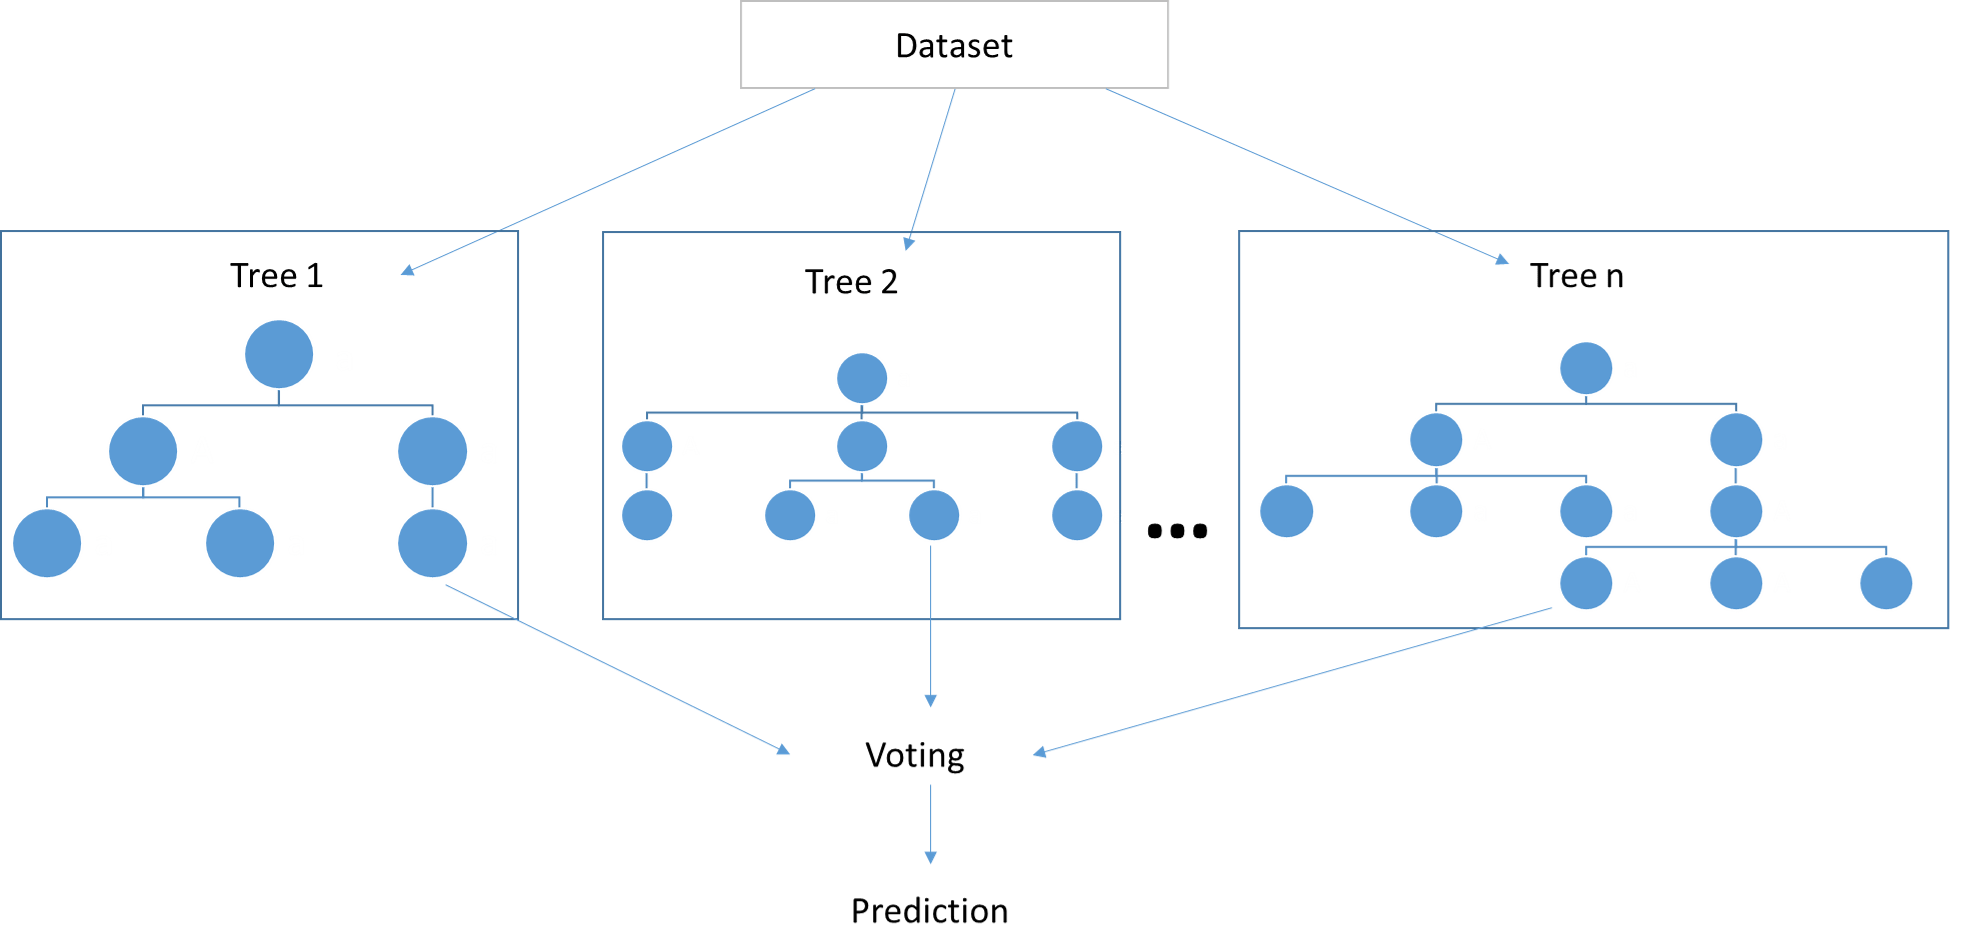
\includegraphics[width=\textwidth]{fig/rf}
Shake the data
\begin{itemize}
\item Shake the rows
\item Shake the columns
\end{itemize}
\url{https://cs.stanford.edu/~karpathy/svmjs/demo/demoforest.html}
}

\begin{frame}[fragile]\frametitle{}
\tiny	
\begin{lstlisting}
import pandas as pd
import numpy as np
path='data/'
filename = path+'spamdata.csv'
spam = pd.read_csv(filename)
\end{lstlisting} 
\pause
\begin{lstlisting}
X = spam.values[:,:57]
y = spam.values[:,57]

from sklearn.model_selection import train_test_split
X_train, X_test, y_train, y_test = 
	train_test_split(X,y, test_size= 0.1)
\end{lstlisting} 
\pause
\begin{lstlisting}
from sklearn.ensemble import RandomForestClassifier
rf = RandomForestClassifier(n_estimators=100)
rf.fit(X_train, y_train)
\end{lstlisting} 

\end{frame}



\section{SVM}
\frame{\frametitle{Perceptron}
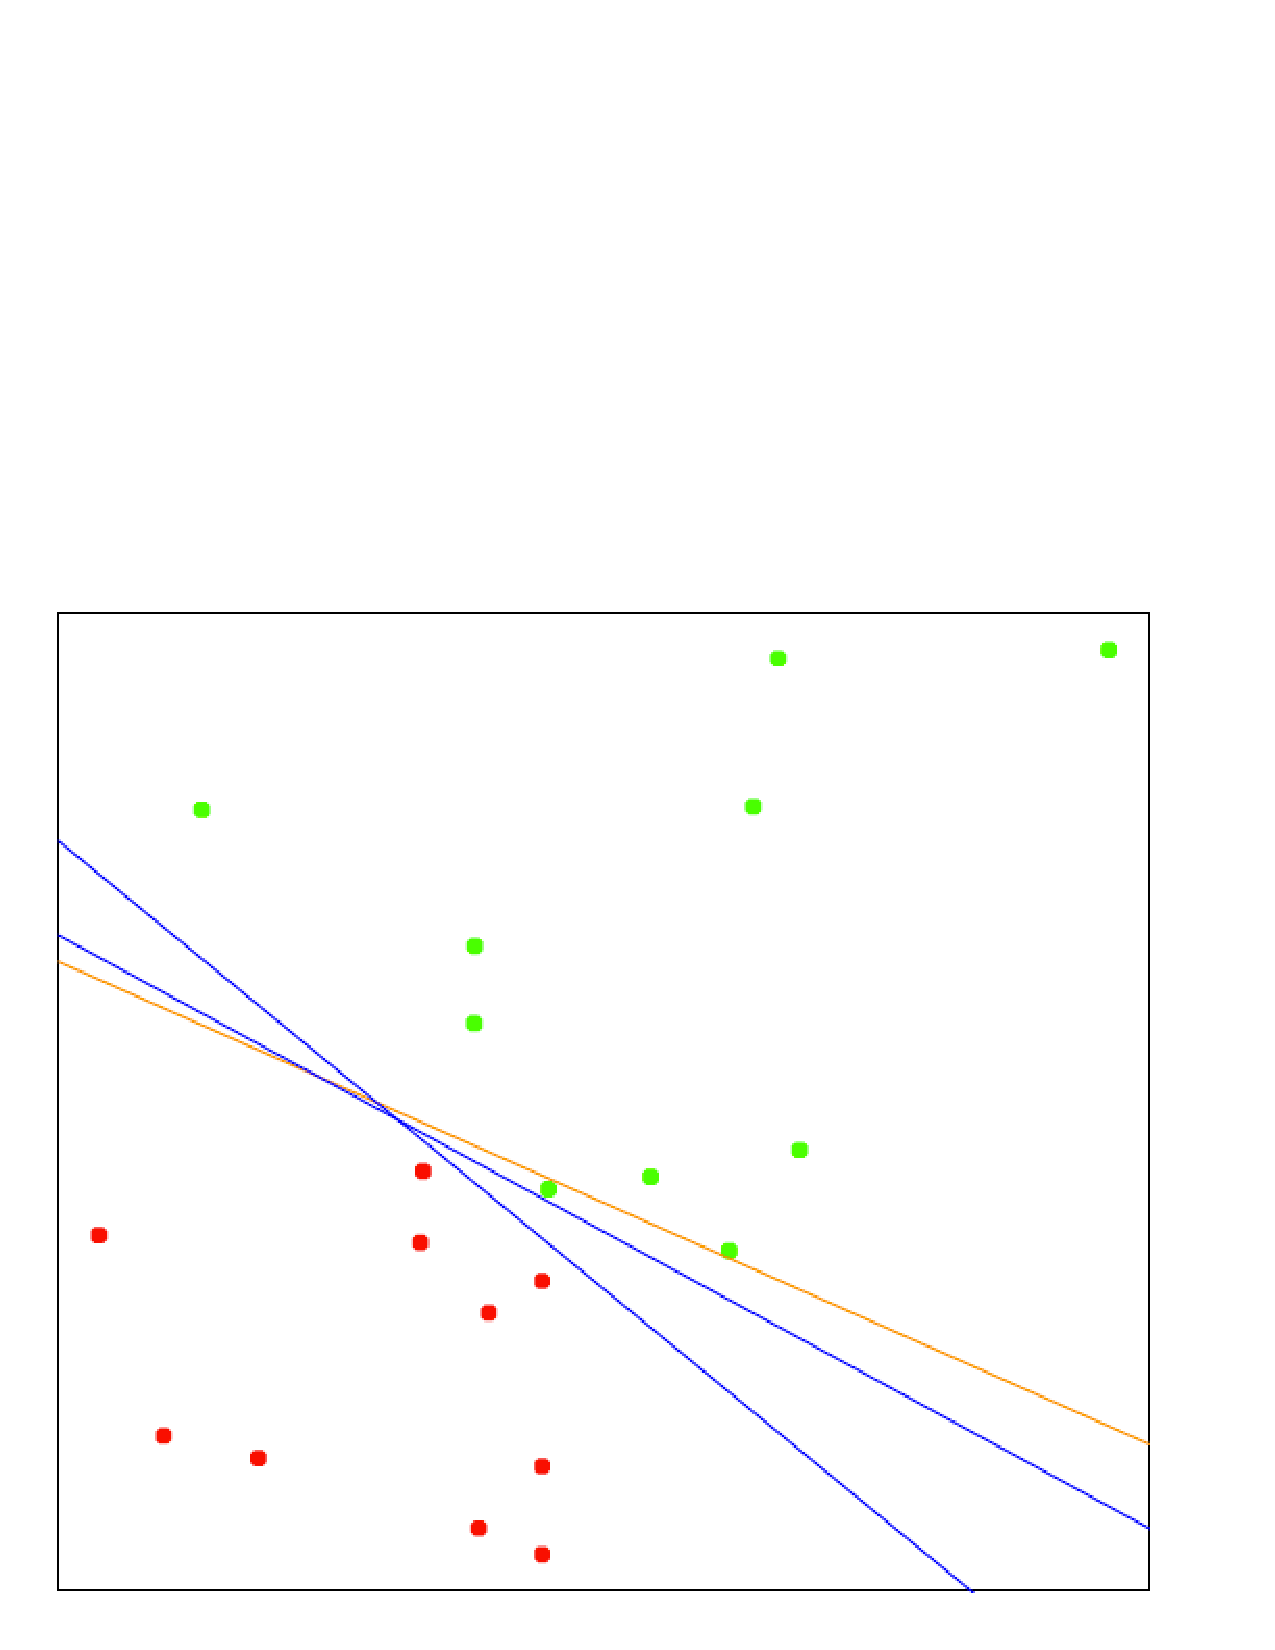
\includegraphics[width=0.45\textwidth]{fig/fig4-14}\pause
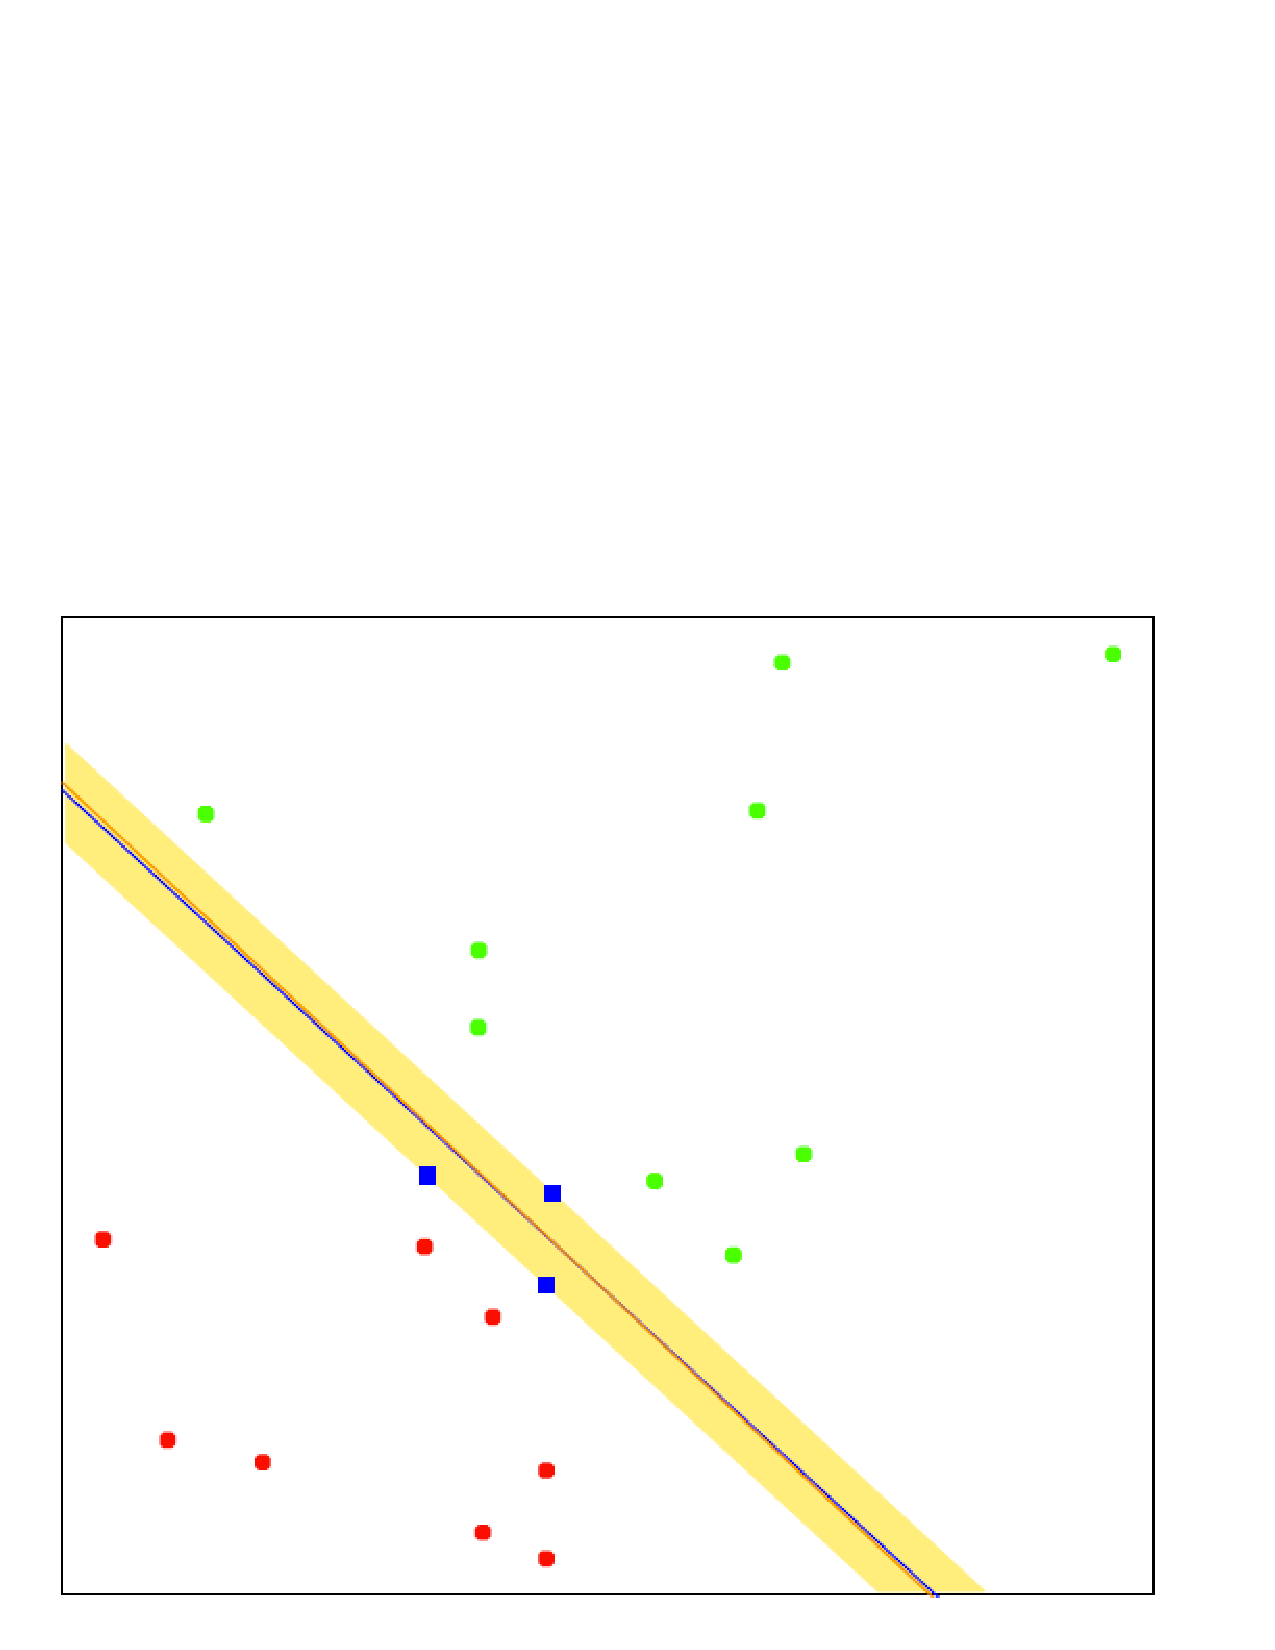
\includegraphics[width=0.45\textwidth]{fig/fig4-16}
}

\frame{\frametitle{Maximum Margin}
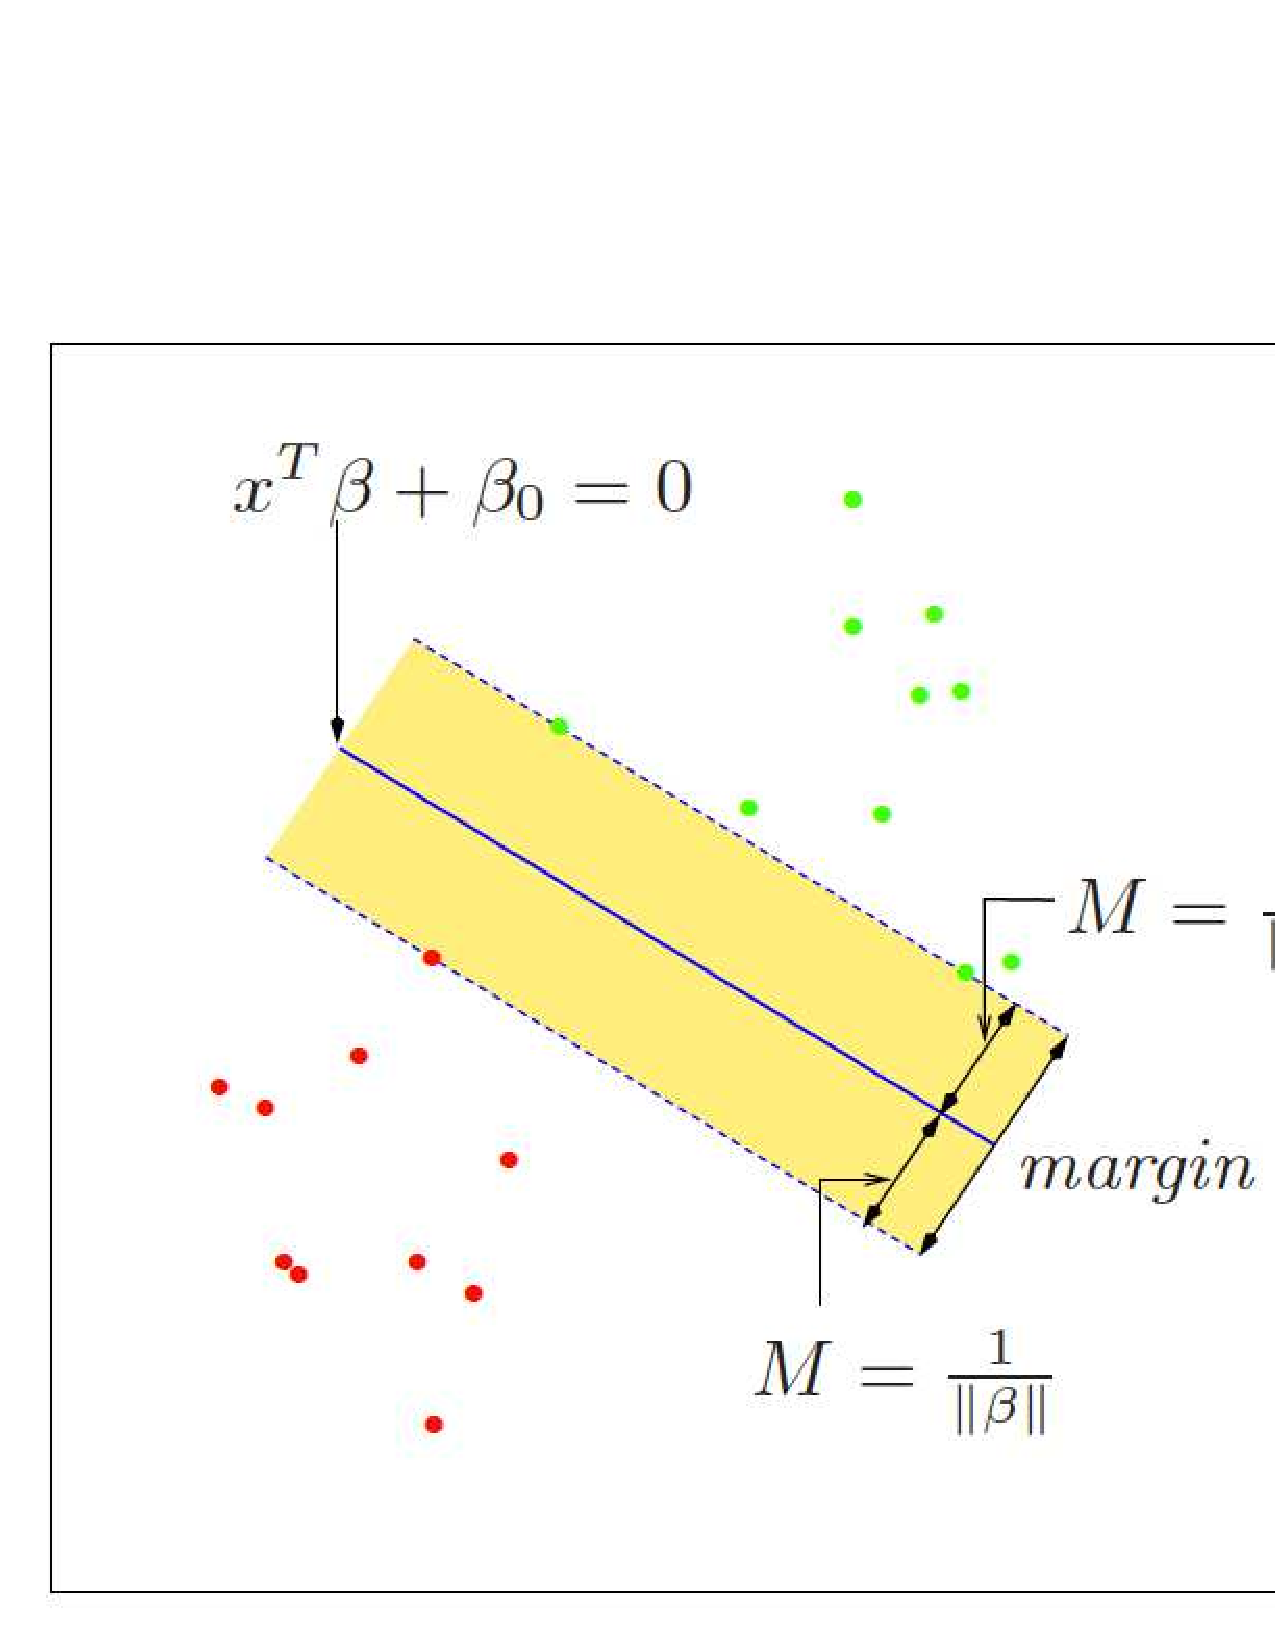
\includegraphics[width=0.45\textwidth]{fig/fig12-1-01}\pause
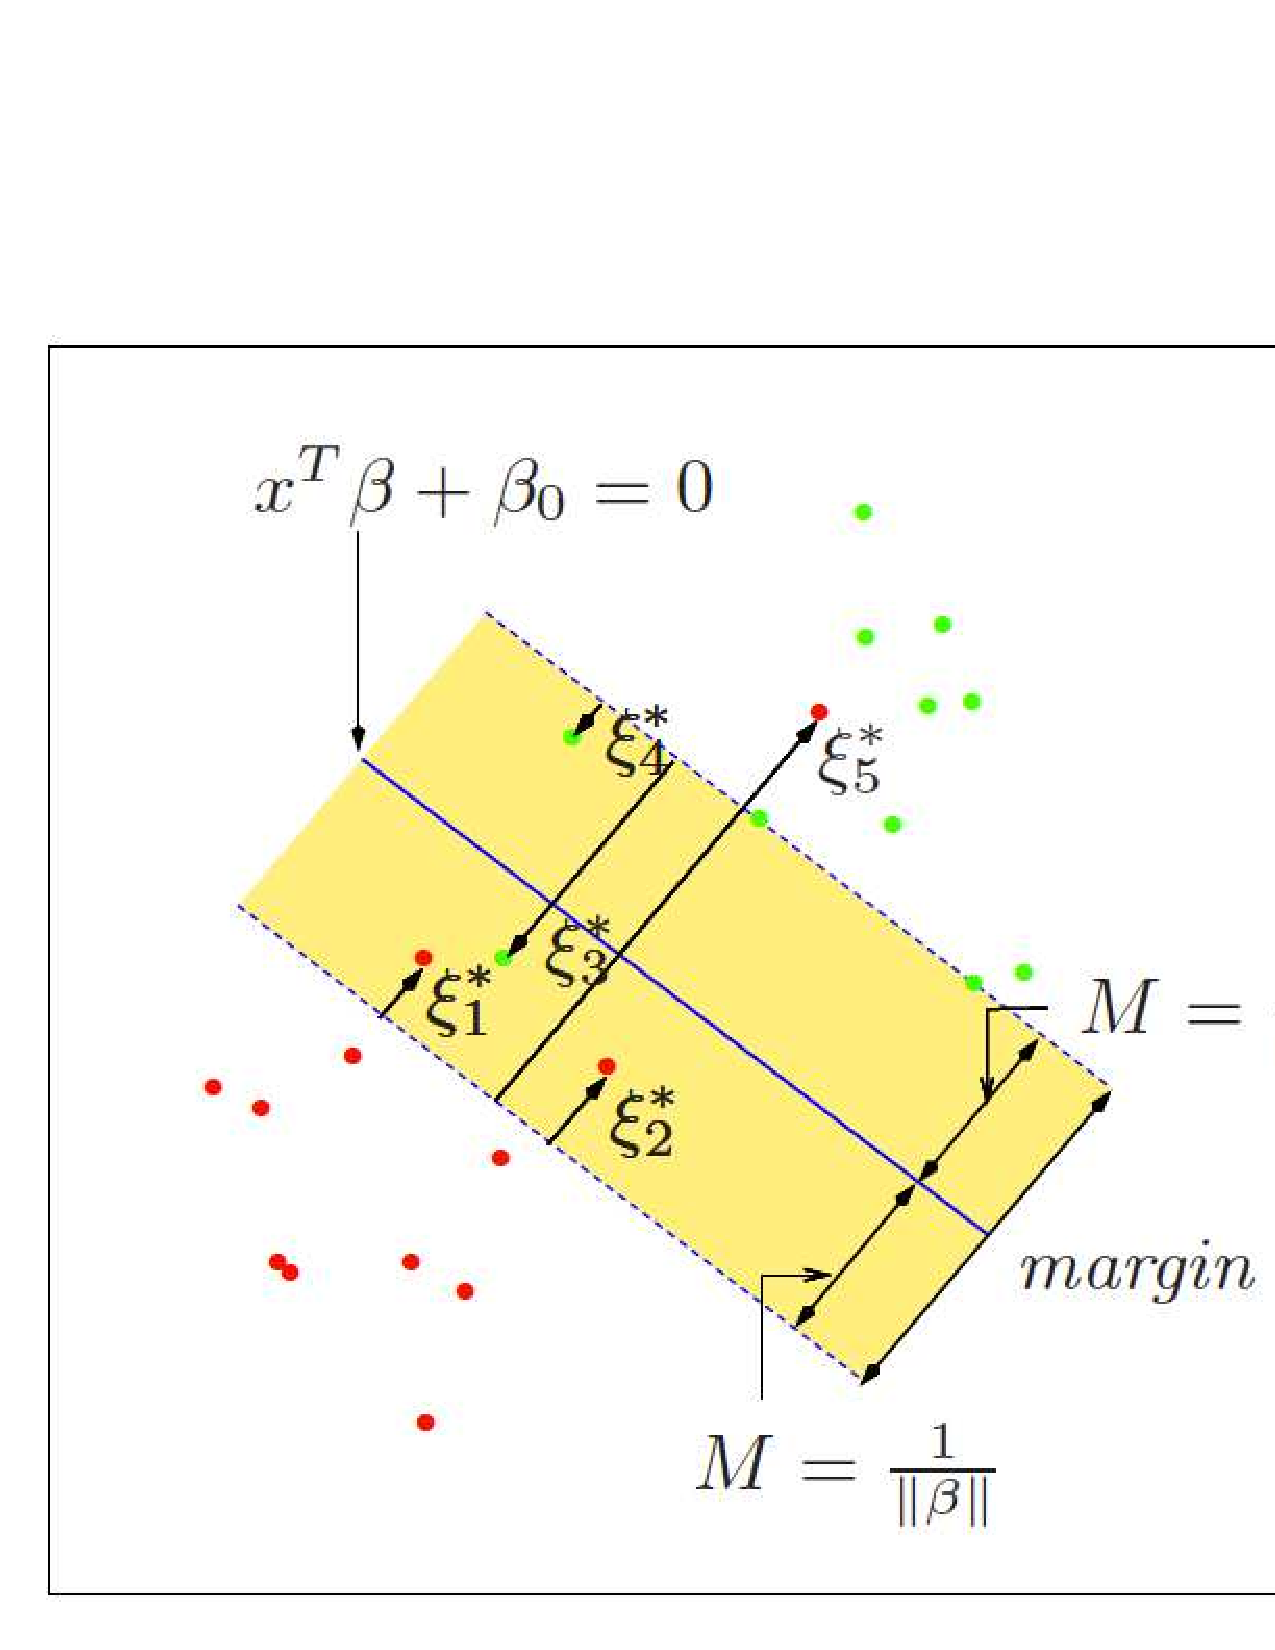
\includegraphics[width=0.45\textwidth]{fig/fig12-1-02}\\
\url{https://cs.stanford.edu/~karpathy/svmjs/demo/}
}

\frame{\frametitle{Kernels}
 \begin{itemize}
\item Linear: $\x\t\y$
 \item Polynomial: $K(\x, \y)= (1+\x\t \y)^d$
\item Radial: $K(\x, \y)= \exp\{ -{1\over \sigma^2} (\x-\y)\t (\x-\y) \} $
\item Neural Network: $K(\x, \y)= \mathrm{tanh} \{b_0 + b_1 \x\t \y \} $
 \end{itemize}
}


\begin{frame}[fragile]\frametitle{}
\tiny	
\begin{lstlisting}
from sklearn.svm import SVC
sv = SVC(C=10)
sv.fit(X_train,y_train)
accuracy_score(sv.predict(X_test), y_test)
\end{lstlisting} 

\end{frame}


\section{Neural Network}
\frame{\frametitle{Perceptron}
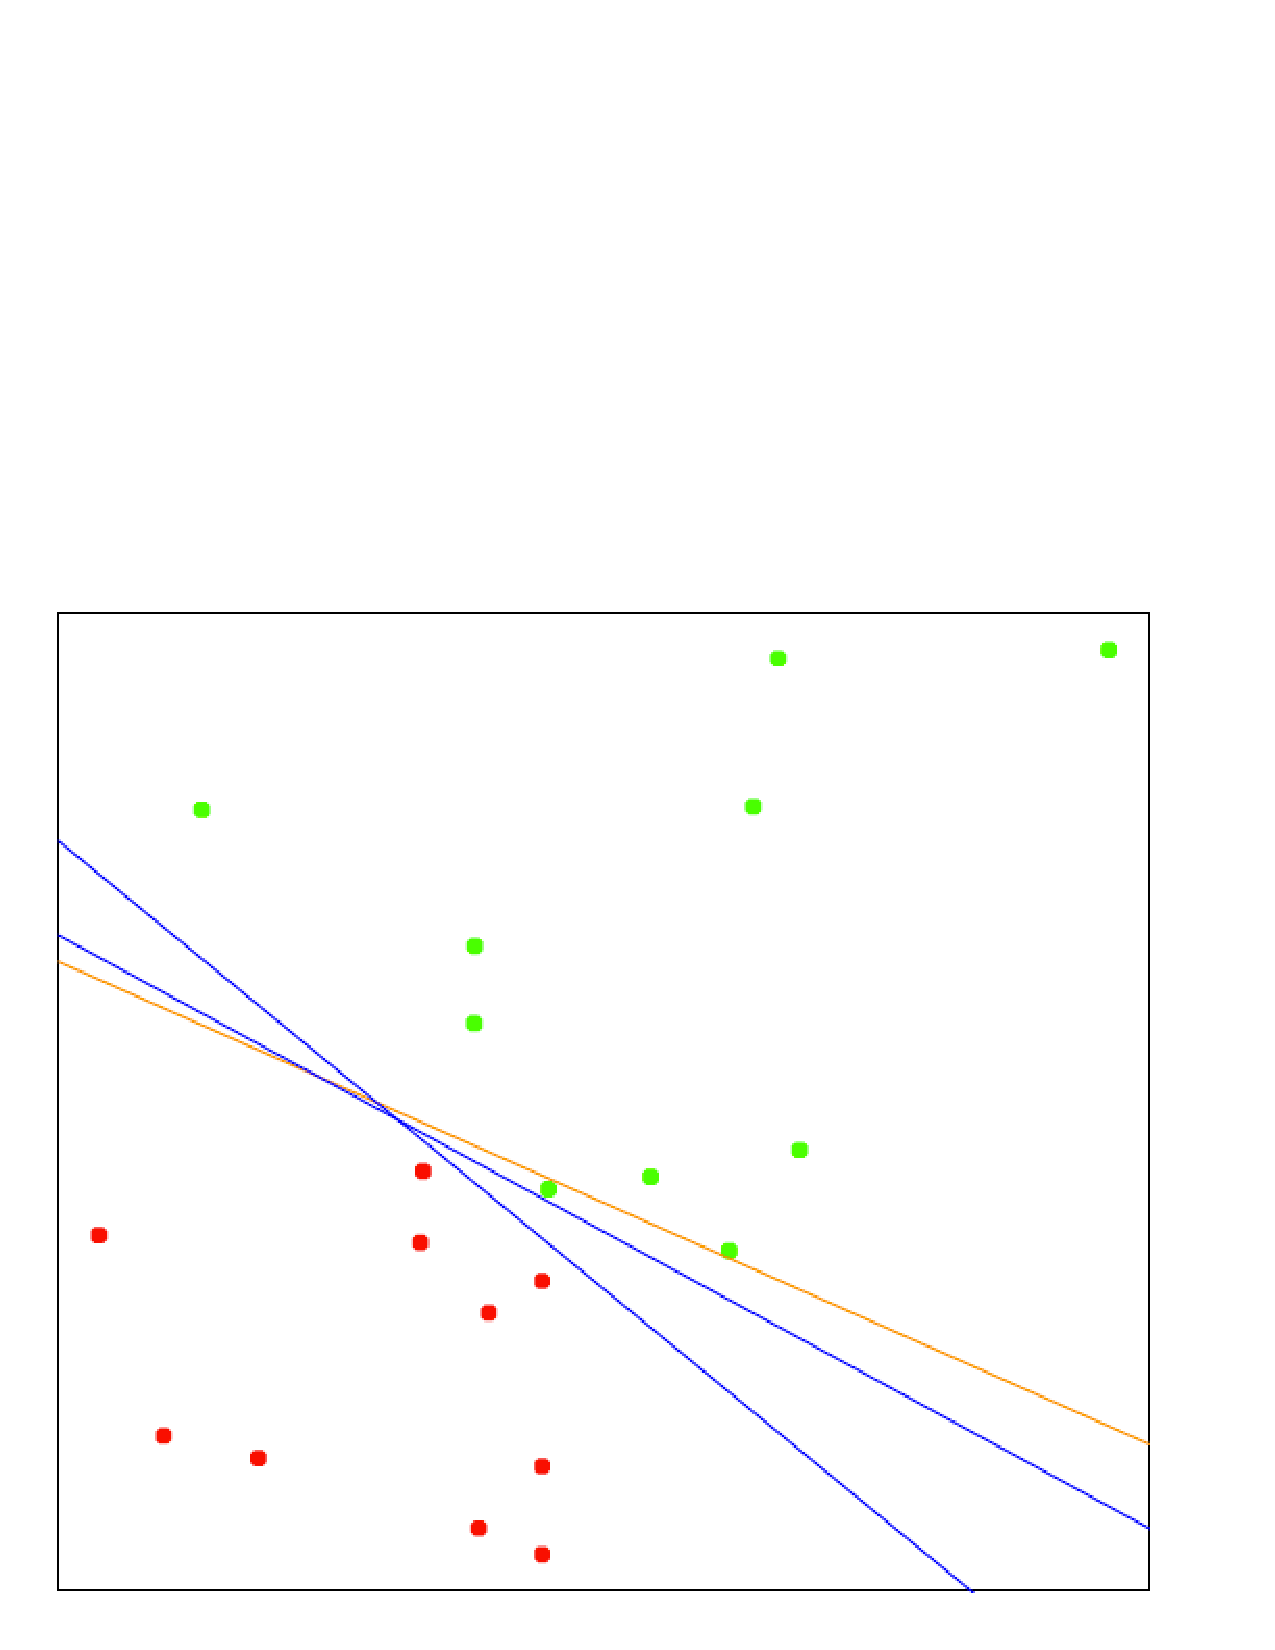
\includegraphics[width=0.45\textwidth]{fig/fig4-14}\pause
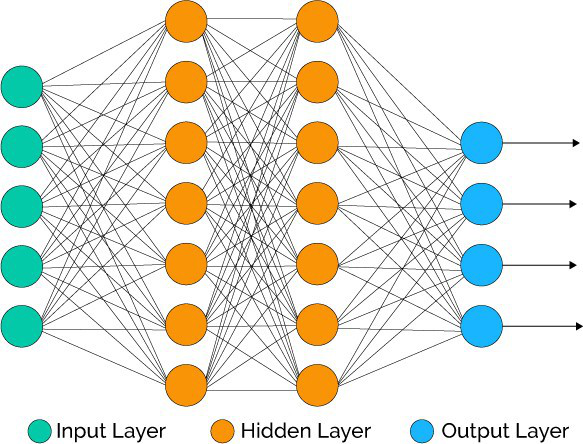
\includegraphics[width=0.45\textwidth]{fig/nn}
}



\begin{frame}[fragile]\frametitle{}
\tiny	
\begin{lstlisting}
from sklearn.neural_network import MLPClassifier
nn = MLPClassifier(hidden_layer_sizes=(10, 10), 
	activation='logistic')
nn.fit(X_train, y_train)
accuracy_score(nn.predict(X_test), y_test)
\end{lstlisting} 
\end{frame}


\section{Zip code}
\frame{\frametitle{Zip code}
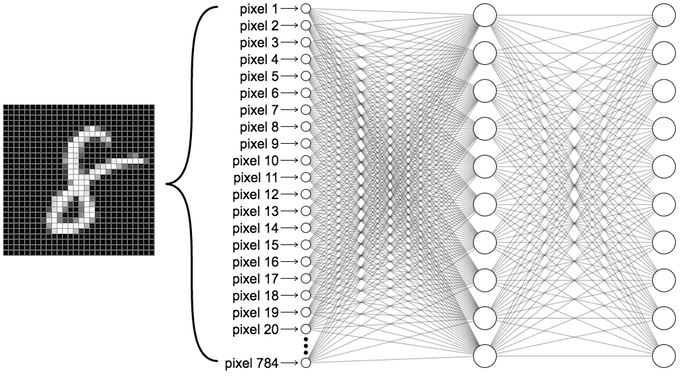
\includegraphics[width=\textwidth]{fig/zipnn}\\
\url{http://scs.ryerson.ca/~aharley/vis/fc/}
}




%\begin{frame}[fragile]\frametitle{}
%\tiny	
%\begin{lstlisting}
%\end{lstlisting} 
%\end{frame}


%\begin{frame}[fragile]\frametitle{}
%\tiny	
%\begin{lstlisting}
%\end{lstlisting} 
%\end{frame}


%\frame{\frametitle{}
%\includegraphics[width=0.5\textwidth]{fig/}
%}

%\frame{\frametitle{}
%\includegraphics[width=0.5\textwidth]{fig/}
%}

%\frame{\frametitle{}
%\includegraphics[width=0.5\textwidth]{fig/}
%}
%
%
%
%

\end{document}
